\documentclass[tikz,border=0cm]{standalone}
\usepackage{type1cm}
\usepackage{fp}
\usetikzlibrary{decorations.pathmorphing}
\usetikzlibrary{calc}
\usetikzlibrary{shadows}


\usepackage{fetamont}
\usepackage{cmbright}

\usepackage{bm,amsmath,amssymb}
\usepackage{soul}

\edef\myfontscale{1.2}
% \definecolor{simula}{RGB}{245,130,32}
% https://intranet.simula.no/sites/default/files/simula_rebrand_readme_2016.pdf
\definecolor{simula}{RGB}{241, 90, 34}
\definecolor{amaranth}{rgb}{0.9, 0.17, 0.31}
\definecolor{amber}{rgb}{1.0, 0.75, 0.0}

%% scalable vector fonts
\edef\fontSizeX{12}\edef\fontSizeY{14}
\FPupn{\resulttinyX}{myfontscale fontSizeX * 2 round}
\FPupn{\resulttinyY}{myfontscale fontSizeY * 2 round}
\renewcommand*{\tiny}{\fontsize{\resulttinyX}{\resulttinyY}\selectfont}

\edef\fontSizeX{14.4}\edef\fontSizeY{18}   
\FPupn{\resultscriptsizeX}{myfontscale fontSizeX * 2 round}
\FPupn{\resultscriptsizeY}{myfontscale fontSizeY * 2 round}
\renewcommand*{\scriptsize}{\fontsize{\resultscriptsizeX}{\resultscriptsizeY}\selectfont}

\edef\fontSizeX{17.28}\edef\fontSizeY{22}
\FPupn{\resultfootnotesizeX}{myfontscale fontSizeX * 2 round}
\FPupn{\resultfootnotesizeY}{myfontscale fontSizeY * 2 round}
\renewcommand*{\footnotesize}{\fontsize{\resultfootnotesizeX}{\resultfootnotesizeY}\selectfont}

\edef\fontSizeX{20.74}\edef\fontSizeY{25}
\FPupn{\resultsmallX}{myfontscale fontSizeX * 2 round}
\FPupn{\resultsmallY}{myfontscale fontSizeY * 2 round}
\renewcommand*{\small}{\fontsize{\resultsmallX}{\resultsmallY}\selectfont}

\edef\fontSizeX{24.88}\edef\fontSizeY{30}
\FPupn{\resultnormalsizeX}{myfontscale fontSizeX * 2 round}
\FPupn{\resultnormalsizeY}{myfontscale fontSizeY * 2 round}
\renewcommand*{\normalsize}{\fontsize{\resultnormalsizeX}{\resultnormalsizeY}\selectfont}

\edef\fontSizeX{29.86}\edef\fontSizeY{37}
\FPupn{\resultlargeX}{myfontscale fontSizeX * 2 round}
\FPupn{\resultlargeY}{myfontscale fontSizeY * 2 round}
\renewcommand*{\large}{\fontsize{\resultlargeX}{\resultlargeY}\selectfont}

\edef\fontSizeX{35.83}\edef\fontSizeY{45}
\FPupn{\resultLargeX}{myfontscale fontSizeX * 2 round}
\FPupn{\resultLargeY}{myfontscale fontSizeY * 2 round}
\renewcommand*{\Large}{\fontsize{\resultLargeX}{\resultLargeY}\selectfont}

\edef\fontSizeX{43}\edef\fontSizeY{54}
\FPupn{\resultLARGEX}{myfontscale fontSizeX * 2 round}
\FPupn{\resultLARGEY}{myfontscale fontSizeY * 2 round}
\renewcommand*{\LARGE}{\fontsize{\resultLARGEX}{\resultLARGEY}\selectfont}

\edef\fontSizeX{51.6}\edef\fontSizeY{64}
\FPupn{\resulthugeX}{myfontscale fontSizeX * 2 round}
\FPupn{\resulthugeY}{myfontscale fontSizeY * 2 round}
\renewcommand*{\huge}{\fontsize{\resulthugeX}{\resulthugeY}\selectfont}

\edef\fontSizeX{61.92}\edef\fontSizeY{77}
\FPupn{\resultHugeX}{myfontscale fontSizeX * 2 round}
\FPupn{\resultHugeY}{myfontscale fontSizeY * 2 round}
\renewcommand*{\Huge}{\fontsize{\resultHugeX}{\resultHugeY}\selectfont}

\edef\fontSizeX{74.3}\edef\fontSizeY{93}
\FPupn{\resultveryHugeX}{myfontscale fontSizeX * 2 round}
\FPupn{\resultveryHugeY}{myfontscale fontSizeY * 2 round}
\newcommand*{\veryHuge}{\fontsize{\resultveryHugeX}{\resultveryHugeY}\selectfont}

\edef\fontSizeX{89.16}\edef\fontSizeY{112}
\FPupn{\resultVeryHugeX}{myfontscale fontSizeX * 2 round}
\FPupn{\resultVeryHugeY}{myfontscale fontSizeY * 2 round}
\newcommand*{\VeryHuge}{\fontsize{\resultVeryHugeX}{\resultVeryHugeY}\selectfont}

\edef\fontSizeX{107}\edef\fontSizeY{134}
\FPupn{\resultVERYHugeX}{myfontscale fontSizeX * 2 round}
\FPupn{\resultVERYHugeY}{myfontscale fontSizeY * 2 round}
\newcommand*{\VERYHuge}{\fontsize{\resultVERYHugeX}{\resultVERYHugeY}\selectfont}

% set the normalfont (default)
\renewcommand*{\normalfont}{\normalsize}
% !TEX root = tesi.tex
\newcommand{\R}{\mathbb{R}}
\newcommand{\Cfield}{\mathbb{C}}
\newcommand{\vect}[1]{\mathbf{#1}}
\newcommand{\tens}[1]{\mathsf{#1}}
% something between bar and overline
%\newcommand{\overbar}[1]{\mkern 1.5mu\overline{\mkern-1.5mu#1\mkern-1.5mu}\mkern 1.5mu}
\makeatletter
\newsavebox\myboxA
\newsavebox\myboxB
\newlength\mylenA
\newcommand*\overbar[2][1.00]{%
    \sbox{\myboxA}{$\m@th#2$}%
    \setbox\myboxB\null% Phantom box
    \ht\myboxB=\ht\myboxA%
    \dp\myboxB=\dp\myboxA%
    \wd\myboxB=#1\wd\myboxA% Scale phantom
    \sbox\myboxB{$\m@th\overline{\copy\myboxB}$}%  Overlined phantom
    \setlength\mylenA{\the\wd\myboxA}%   calc width diff
    \addtolength\mylenA{-\the\wd\myboxB}%
    \ifdim\wd\myboxB<\wd\myboxA%
       \rlap{\hskip 0.5\mylenA\usebox\myboxB}{\usebox\myboxA}%
    \else
        \hskip -0.5\mylenA\rlap{\usebox\myboxA}{\hskip 0.5\mylenA\usebox\myboxB}%
    \fi}
\makeatother

\newcommand{\vx}{\vect{x}}
\newcommand{\vy}{\vect{y}}
\newcommand{\vX}{\vect{X}}
\newcommand{\vA}{\vect{A}}
\newcommand{\va}{\vect{a}}
\newcommand{\vvb}{\vect{b}}
\newcommand{\vc}{\vect{c}}
\newcommand{\vk}{\vect{k}}
\newcommand{\ve}{\vect{e}}
\newcommand{\vp}{\vect{p}}
\newcommand{\vu}{\vect{u}}
\newcommand{\vv}{\vect{v}}
\newcommand{\vb}{\vect{b}}
\newcommand{\vf}{\vect{f}}
\newcommand{\vs}{\vect{s}}
\newcommand{\vg}{\vect{g}}
\newcommand{\vn}{\vect{n}}
\newcommand{\vm}{\vect{m}}
\newcommand{\vh}{\vect{h}}
\newcommand{\vt}{\vect{t}}
\newcommand{\vw}{\vect{w}}
\newcommand{\vfo}{\vf_\circ}
\newcommand{\vso}{\vs_\circ}
\newcommand{\vno}{\vn_\circ}

\newcommand{\vxi}{\bm{\xi}}

\newcommand{\tF}{\tens{F}}
\newcommand{\tT}{\tens{T}}
\newcommand{\tP}{\tens{P}}
\newcommand{\tS}{\tens{S}}
\newcommand{\tI}{\tens{I}}
\newcommand{\tQ}{\tens{Q}}
\newcommand{\tB}{\tens{B}}
\newcommand{\tC}{\tens{C}}
\newcommand{\tE}{\tens{E}}
\newcommand{\tR}{\tens{R}}
\newcommand{\tU}{\tens{U}}
\newcommand{\tA}{\tens{A}}
\newcommand{\tD}{\tens{D}}
\newcommand{\tH}{\tens{H}}
\newcommand{\tJ}{\tens{J}}
\newcommand{\tX}{\tens{X}}
\newcommand{\tV}{\tens{V}}
\newcommand{\tM}{\tens{M}}
\newcommand{\tL}{\tens{L}}

\newcommand{\tFiso}{\tF_\mathsf{iso}}
\newcommand{\tFvol}{\tF_\mathsf{vol}}

\newcommand{\tTiso}{\tT_\mathsf{iso}}
\newcommand{\btTiso}{\overbar[0.75]{\tT}_\mathsf{iso}}
\newcommand{\tTvol}{\tT_\mathsf{vol}}

\newcommand{\tSiso}{\tS_\mathsf{iso}}
\newcommand{\btSiso}{\overbar[0.9]{\tS}_\mathsf{iso}}
\newcommand{\tSvol}{\tS_\mathsf{vol}}

\newcommand{\tCiso}{\tC_\mathsf{iso}}
\newcommand{\tEiso}{\tE_\mathsf{iso}}
\newcommand{\tBiso}{\tB_\mathsf{iso}}
\newcommand{\vfiso}{\vf_\mathsf{iso}}
\newcommand{\vsiso}{\vs_\mathsf{iso}}
\newcommand{\cIiso}{\cI^\mathsf{iso}}

\newcommand{\tFa}{\tF_\mathsf{a}}
\newcommand{\tFe}{\tF_\mathsf{e}}
\newcommand{\tauref}{\tau_{\textsf{ref}}}
\newcommand{\tPa}{\tP_\mathsf{a}}
\newcommand{\tPe}{\tP_\mathsf{e}}
\newcommand{\tTa}{\tT_\mathsf{a}}
\newcommand{\tTe}{\tT_\mathsf{e}}
\newcommand{\tSa}{\tS_\mathsf{a}}
\newcommand{\tSe}{\tS_\mathsf{e}}
\newcommand{\tBe}{\tB_\mathsf{e}}
\newcommand{\tCe}{\tC_\mathsf{e}}

\newcommand{\sSa}{s_\mathsf{a}}
\newcommand{\bsSa}{\overbar s_\mathsf{a}}

\newcommand{\htSa}{\widehat\tS_\textsf{a}}

\newcommand{\body}{\mathfrak{B}}

\newcommand{\vphi}{\bm{\varphi}}
\newcommand{\veta}{\bm{\eta}}
\newcommand{\vvphi}{\hm{\varphi}}
\newcommand{\vTheta}{\bm{\Theta}}
\newcommand{\vpp}{\mathbf{p}}

\newcommand{\tK}{\tens{K}}
\newcommand{\tO}{\tens{O}}
\newcommand{\tKuu}{\tK_\mathsf{\varphi\varphi}}
\newcommand{\tKup}{\tK_\mathsf{\varphi p}}
\newcommand{\tKpu}{\tK_\mathsf{p \varphi}}
\newcommand{\tKpt}{\tK_\mathsf{p \theta}}
\newcommand{\tKtp}{\tK_\mathsf{\theta p}}
\newcommand{\tKtt}{\tK_\mathsf{\theta\theta}}
\newcommand{\tKpp}{\tK_\mathsf{pp}}
\newcommand{\vrhs}{\bm{\mathsf{f}}}
\newcommand{\vrhsu}{\vrhs_\mathsf{\varphi}}
\newcommand{\vrhst}{\vrhs_\mathsf{\theta}}
\newcommand{\vrhsp}{\vrhs_\mathsf{p}}

\newcommand{\cW}{\mathcal{W}}
\newcommand{\hcW}{\widehat\cW}
\newcommand{\tcW}{\widetilde\cW}
\newcommand{\hcWorth}{\hcW_\mathsf{orth}}
\newcommand{\hcWtr}{\hcW_\mathsf{tr}}
\newcommand{\cWiso}{\cW_\mathsf{iso}}
\newcommand{\hcWiso}{\hcW_\mathsf{iso}}
\newcommand{\cWvol}{\cW_\mathsf{vol}}
\newcommand{\cG}{\mathscr{G}}
\newcommand{\cGorth}{\cG_\mathsf{orth}}
\newcommand{\cGtr}{\cG_\mathsf{tr}}

\newcommand{\cI}{\mathcal{I}}

\newcommand{\aaf}{a_\mathsf{f}}
\newcommand{\aas}{a_\mathsf{s}}
\newcommand{\bbf}{b_\mathsf{f}}
\newcommand{\bbs}{b_\mathsf{s}}
\newcommand{\aafs}{a_\mathsf{fs}}
\newcommand{\bbfs}{b_\mathsf{fs}}

\newcommand{\CC}{\mathbb{C}}
\newcommand{\CCiso}{\CC_\mathsf{iso}}
\newcommand{\cc}{\mathfrak{c}}
\newcommand{\cciso}{\cc_\mathsf{iso}}
\newcommand{\ccvol}{\cc_\mathsf{vol}}
\newcommand{\bcciso}{\overbar{\cc}_\mathsf{iso}}

\newcommand{\tsp}[1]{#1^\mathsf{T}}
\newcommand{\mtsp}[1]{#1^{-\mathsf{T}}}
\newcommand{\dd}{\mathrm{d}}
\newcommand{\DD}{\mathrm{D}}

\newcommand{\eps}{\varepsilon}

\newcommand{\bracket}[1]{\left\langle #1 \right\rangle}
\newcommand{\norm}[1]{\left\Vert #1 \right\Vert}

\newcommand{\Piext}{\Pi_\mathsf{ext}}

\newcommand{\Lin}{\mathrm{Lin}}
\newcommand{\Linp}{\mathrm{Lin}^+}
\newcommand{\Orth}{\mathrm{Orth}}
\newcommand{\Orthp}{\mathrm{Orth}^+}
\newcommand{\Symp}{\mathrm{Sym}^+}

\newcommand{\ddV}{\dd V}
\newcommand{\ddv}{\dd v}
\newcommand{\ddA}{\dd A}
\newcommand{\dda}{\dd a}

\newcommand{\Vinner}{V_\mathsf{inner}}
\newcommand{\pinner}{p_\mathsf{inner}}

%\DeclareMathOperator{\diver}{div}
%\DeclareMathOperator{\tr}{tr}
%\DeclareMathOperator{\cof}{cof}
%\DeclareMathOperator{\dev}{dev}
%\DeclareMathOperator{\vol}{vol}
%\DeclareMathOperator{\DIV}{\textsc{Div}}
%\DeclareMathOperator{\DEV}{\textsc{Dev}}
%\DeclareMathOperator{\GRAD}{\textsc{Grad}}
%\DeclareMathOperator{\sym}{sym}
%\DeclareMathOperator{\diag}{diag}
%\DeclareMathOperator{\sign}{sign}

%\DeclareMathOperator*{\esssup}{ess\kern3pt sup}

\newcommand{\fcubic}{f_\mathsf{cubic}}
\newcommand{\fstep}{f_\mathsf{step}}
%\DeclareMathOperator{\Heavi}{\mathcal{H}}

\newcommand{\Cm}{C_\textsf{m}}
\newcommand{\Iionic}{I_\textsf{ionic}}
\newcommand{\Isource}{I_\textsf{source}}



\usepackage{booktabs,dcolumn}
\usepackage{array}
\newcolumntype{T}{>{\begingroup\bfseries}r<{\endgroup}}
\newcolumntype{N}{D{.}{.}{-1}}
\newcolumntype{R}{D{.}{.}{2.4}}
\newcolumntype{K}{D{.}{.}{3.4}}
\newcommand{\imgcase}[2]{\includegraphics[width=0.5\linewidth]{#1_#2_base}%
\includegraphics[width=0.5\linewidth]{#1_#2_side}}
\usepackage[tableposition=top,font=footnotesize,labelfont=bf,sf]{caption}

\usepackage[margin=1in, paperwidth=48in, paperheight=48in]{geometry}

\begin{document}
% A1 poster, see https://www.prepressure.com/library/paper-size#ISO
\begin{tikzpicture}[x=23.39in, y=33.11in]
\fill[white, use as bounding box] (0, 0) rectangle (1, 1);

%%%% title %%%%
\begingroup
\pgfmathsetseed{3674}
\node[decoration={random steps, segment length=1cm, amplitude=3mm}, decorate,
      fill=simula, inner sep=1cm,
      drop shadow={shadow yshift=1ex, shadow xshift=-1ex},
      anchor=north, draw=none, line width=0mm]
      (title)
      at ($(current bounding box.north)-(0,2.5cm)$)
  {\begin{minipage}{20in}
   \begin{center}
   {\ffmfamily\bfseries\color{black}
   {\LARGE Inverse estimation of physiological parameters from brain anatomical changes}} \\[0.4ex]
   \bigskip
   {\color{white}
   \textbf{\underline{Henrik Finsberg}\textsuperscript{1}, Anders M. Dale\textsuperscript{2}, Marie E. Rognes\textsuperscript{3}}
   }

   %\vskip-5mm\footnotesize
   %\texttt{\{sjurug,hake,simonep,sundnes,samwall\}@simula.no}}
   
   \medskip
   \textsuperscript{1}Department of Computational Physiology, Simula Research Laboratory, 0164 Oslo, Norway \\
    \textsuperscript{2} Department of Radiology, University of California San Diego School of Medicine, La Jolla, CA, USA \\
    \textsuperscript{3}Department of Numerical Analysis and Scientific Computing, Simula Research Laboratory, 0164 Oslo, Norway \\
   \end{center}
  \end{minipage}};
\endgroup

%%%% introduction %%%%
\node[anchor=north west]
(motif title)
at ($(current bounding box.north west)+(2cm,-14cm)$)
{\bfseries\ffmfamily\Large\underline{Introduction}};

\node[draw=none, anchor=north west]
(motif text)
at ( $(motif title.south west)+(1cm,0)$ )
{\begin{minipage}{21in}
\footnotesize
\begin{minipage}[t]{0.31\textwidth}
Mild Cognitive Impairment (MCI) signifies a condition where a noticeable reduction in cognitive capabilities can be observed. It is often regarded as an intermediary phase between the expected cognitive decline that accompanies aging and more severe conditions like dementia, including Alzheimer's disease. Because MCI is a
\end{minipage}\hfill
\begin{minipage}[t]{0.31\textwidth}
condition that can lead to dementia, many studies are focusing on it to find possible ways to prevent it. This is primarily due to the fact that adults who receive an MCI diagnosis are more prone to developing Alzheimer's Disease (AD)[4]. In the present study, we leverage longitudinal data from MCI individuals to generate deformation
\end{minipage}\hfill
\begin{minipage}[t]{0.31\textwidth}
maps that are relative to the MRI image from the initial time point. Subsequently, we employ inverse modeling to calculate various mechanical properties such as ventricular pressure and material stiffness. The ultimate goal is understand whether pressure alone can explain the morphological changes observed in the data.
\end{minipage}
\end{minipage}};


\node[draw=simula, line width=1mm, anchor=north west,
      rounded corners=4mm, inner sep=1cm,
      fill=simula!10!white, minimum height=16cm]
(optflow)
at ( $(motif text.south west)-(1cm,1cm)$ )
{\begin{minipage}{9in}
\vspace{0.5cm}
\vfill
\footnotesize
We consider a sequence of 3D structurual MRI images $V^{m} (m = 1, 2, \cdots , M)$ acquired from the same individual at different points in time. All images are registered based on the first image by means of the method described in [1] so that we have a sequence of displacement fields $\mathbf{u}^m, (m = 1, 2, \cdots , M)$ representing the amount of deformation relative to the reference image at the first time point.
\begin{minipage}[t]{9in}
\vspace{0pt}
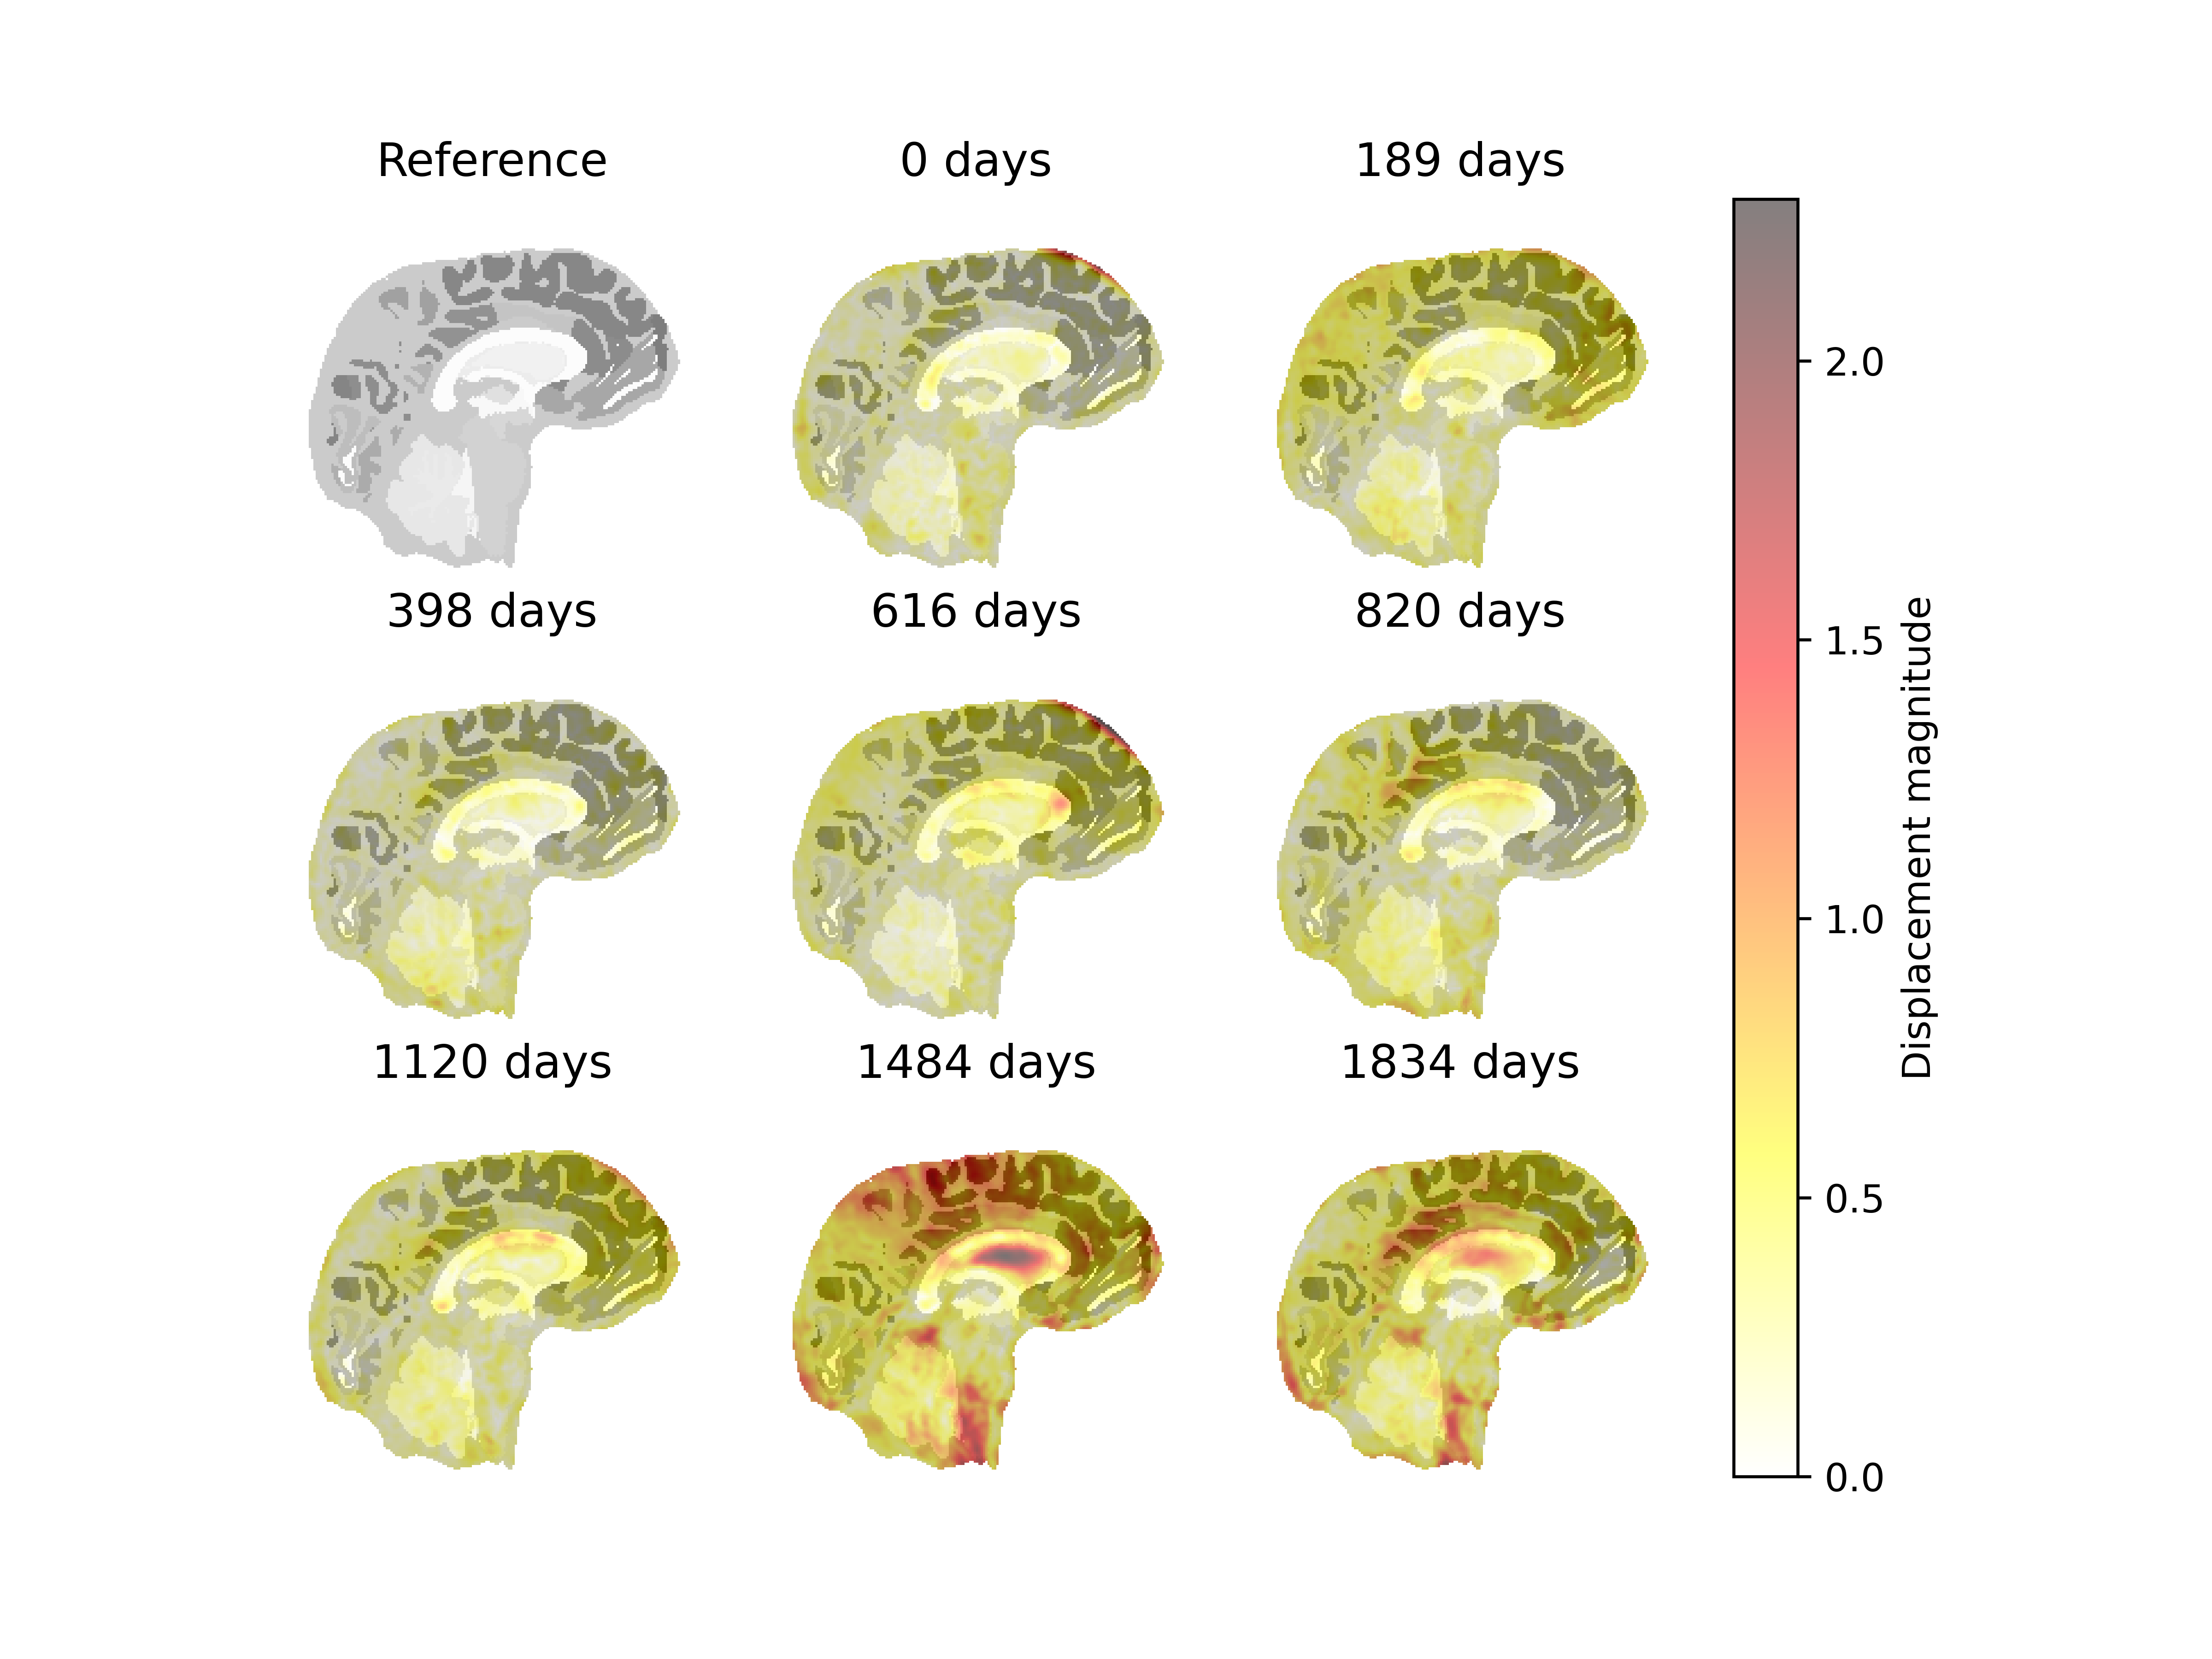
\includegraphics[width=\textwidth]{figures/multiple_times.png}
\end{minipage}\hfill
\begin{minipage}[t]{8.5in}
\vspace{5mm}
\bigskip
\textbf{$\triangle$ Figure:}
Showing slices of 3D MRI images taken of the same individual at different time points. Colormap represent the amount of displacement magnitude relavtive to the reference image at the first time point.
\end{minipage}
\end{minipage}};

\node[anchor=east, rounded corners=3mm, fill=simula]
(optflow title)
at ($ (optflow.north east)!3cm!(optflow.north west) $)
{\ffmfamily Longitudinal MRI scans};

%%%% Feature calculation %%%%
\node[draw=simula, line width=1mm, anchor=north west,
      rounded corners=4mm, inner sep=1cm,
      fill=simula!10!white, minimum height=10cm]
(feature)
at ($(optflow.north east)+(1cm,0)$)
{\begin{minipage}{10.5in}
\footnotesize

We model the brain parenchyma as a hyperelastic material, solving for a displacement field $\mathbf{u}: \Omega \times [t_1, t_2] \mapsto \mathbb{R}^3$. Furthermore, we assume that the deformation gradient $\mathbf{F}$ can be decomposed into a an elastic part $\mathbf{F}_e$ and an atrophy part $\mathbf{F}_a$ with  $\mathbf{F} = \mathbf{F}_e \mathbf{F}_a$, where $\mathbf{F}_a = \sqrt[3]{\theta} \mathbf{I}$ and $\theta = \theta(\mathbf{X}, t)$ is a measure of volume loss [5].

\begin{minipage}[t]{0.4\textwidth}
\vspace{0pt}
\begin{center}
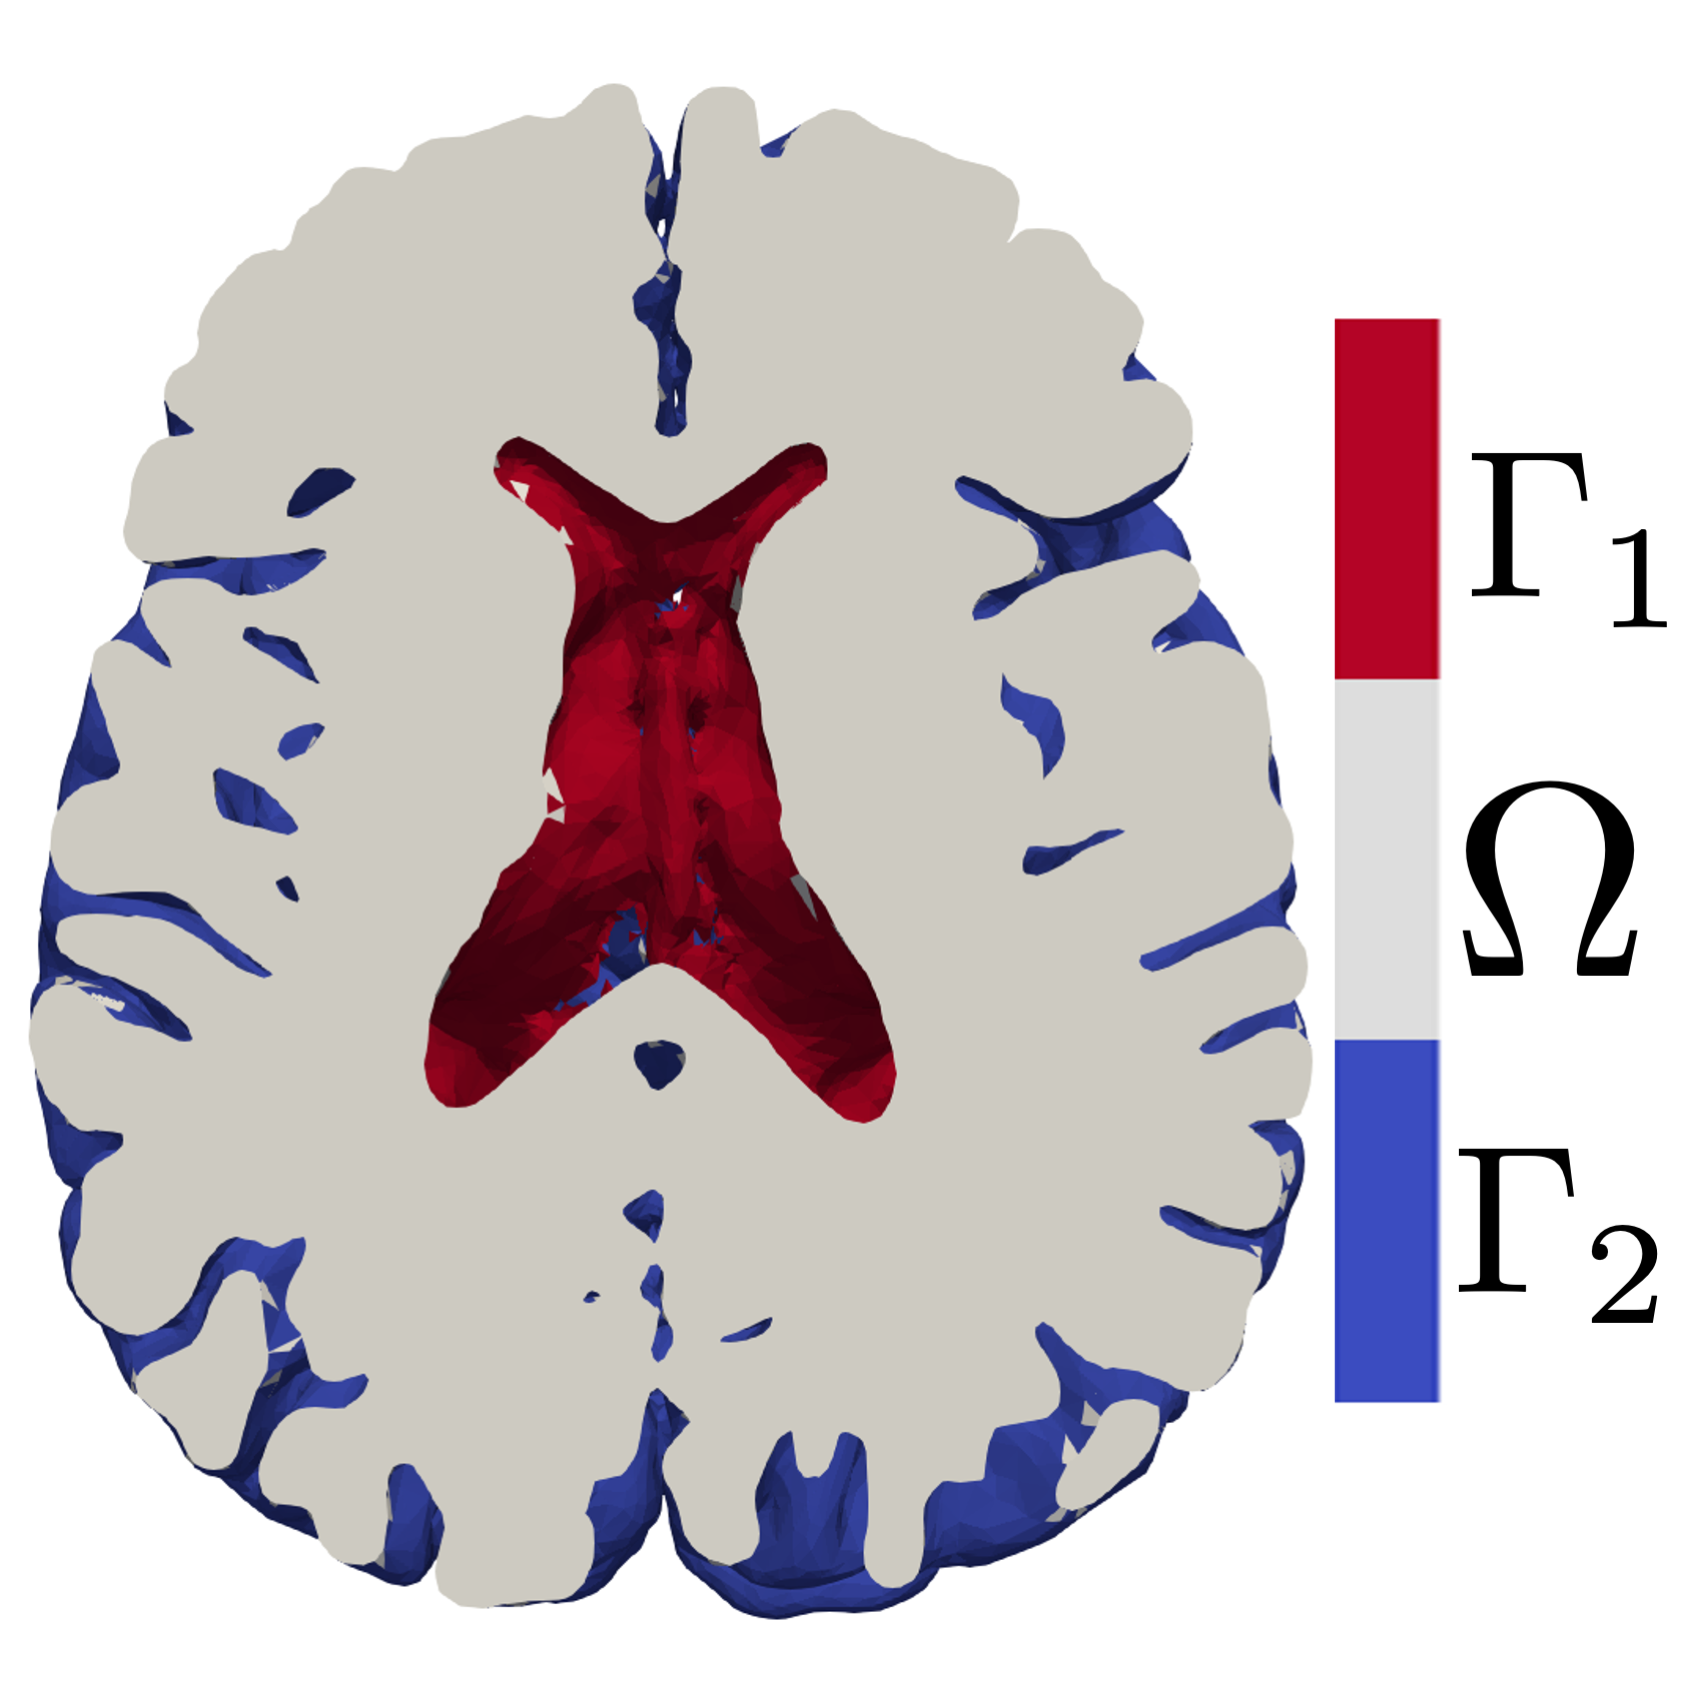
\includegraphics[width=\textwidth]{figures/boundaries.png}    
\end{center}
\textbf{$\triangle$ Figure:}
Showing the interior ($\Omega$), the inner ventricular surface ($\Gamma_1$) and the outer surface $\Gamma_2$.
\end{minipage}\hfill
\begin{minipage}[t]{0.55\textwidth}
\vspace{5mm}

We solve for the balance of linear momentum

\begin{equation}
    \nabla \cdot \mathbf{P} = 0, \quad \mathbf{x} \in \Omega,
    \label{eq:balanace_momentum}
\end{equation}
with $\mathbf{P} = \frac{\partial \Psi}{\partial \mathbf{F}}$  
\begin{equation}
    \Psi = \frac{\mu}{2}\left(\mathbf{F}_e : \mathbf{F}_e - 3 - 2 \ln{\det{\mathbf{F}_e}} \right) + \frac{\lambda}{2} \ln^2{\mathbf{F}_e}
\end{equation}
A pressure field is applied to the inner, ventricular surface
\begin{equation}
    \sigma (\mathbf{u}) \cdot n = - p_0 n, \quad \mathbf{x} \in \Gamma_1,
\end{equation}
and a rigid Dirichlet boundary condition is applied on the outer surface
\begin{equation}
    \mathbf{u} = 0 , \quad \mathbf{x} \in \Gamma_2.
\end{equation}

\end{minipage}


\end{minipage}};

\node[anchor=west, rounded corners=3mm, fill=simula]
(feature title)
at ($ (feature.north west)!3cm!(feature.north east) $)
{\ffmfamily Forward modeling};

%%%% Sensitivity analysis %%%%
\node[draw=simula, line width=1mm, anchor=north west,
      rounded corners=4mm, inner sep=1cm,
      fill=simula!10!white, minimum height=6in]
(sensitivity)
at ($(optflow.south west)+(0,-2cm)$)
{\begin{minipage}{9in}
\footnotesize
 Triangulated meshes are generated using a semi-automatic pipeline

\begin{minipage}[t]{9in}
\vspace{0pt}
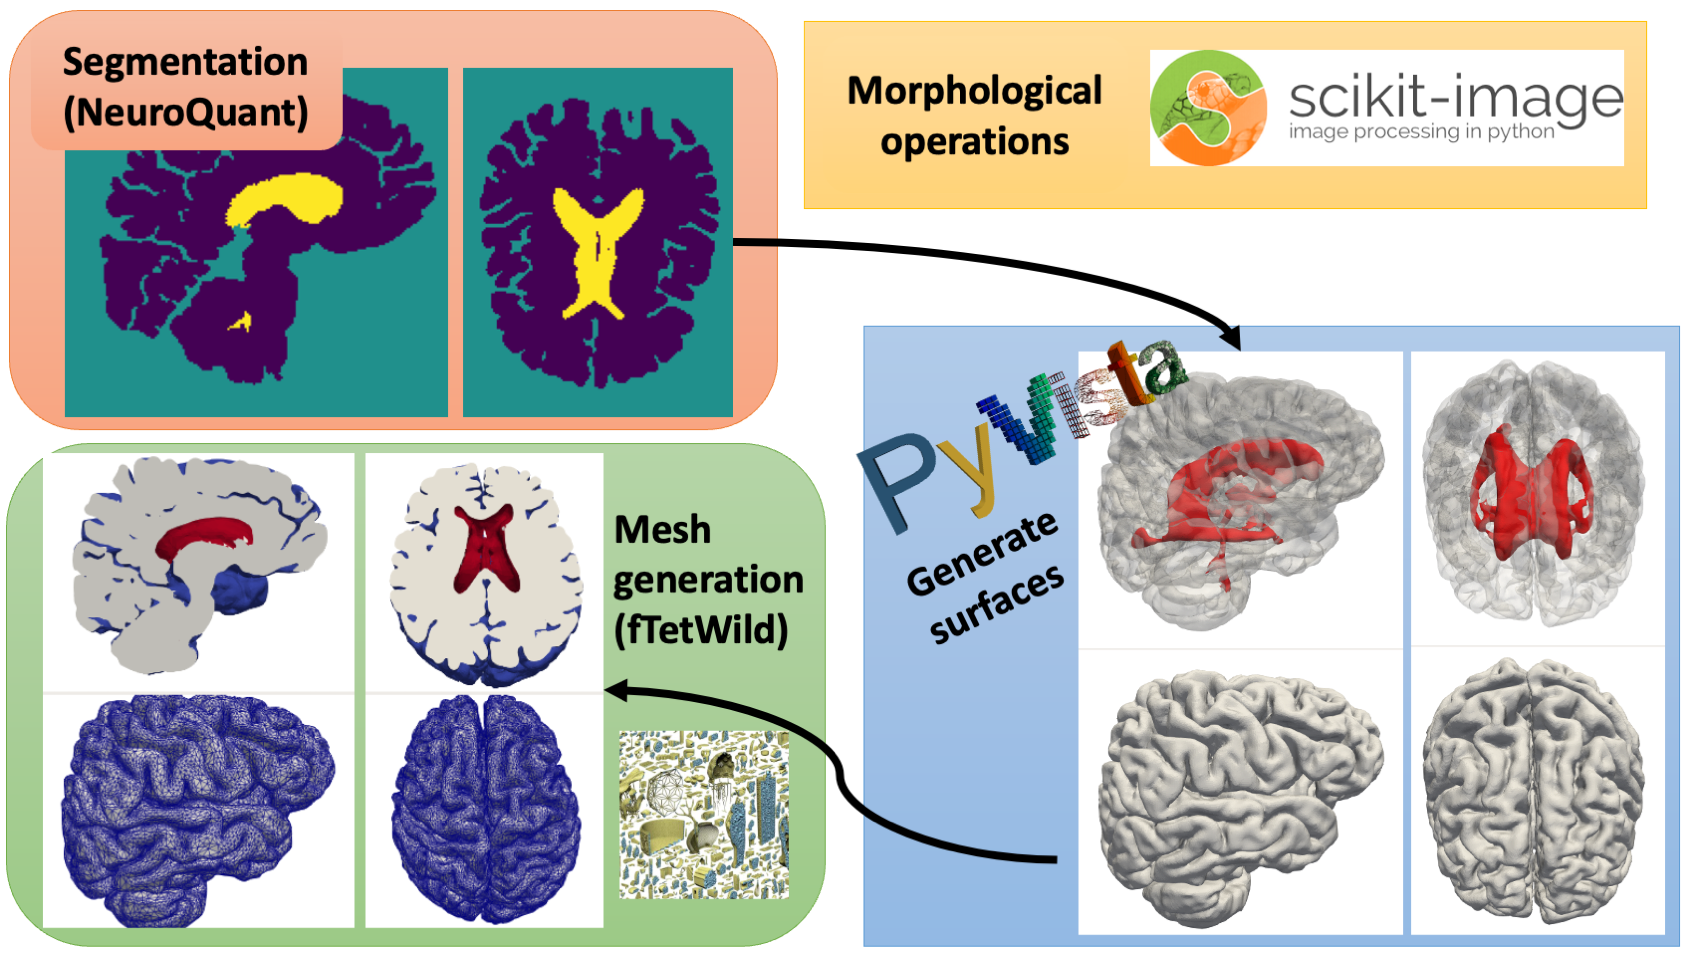
\includegraphics[width=\textwidth]{figures/meshgen.png}
\end{minipage}\hfill
\begin{minipage}[t]{8.5in}
\vspace{5mm}
\bigskip
\textbf{$\triangle$ Figure:}
The 3D voxel images are segmented into regions using NeuroQuant. We generated triagulated surfaces by first thresholding and applying moropholical operations using \emph{scikit-image} and then extractig the surfaces using \emph{pyvista}. We extract the surfaces of the brain parenchyma as well as the vetricles and generate meshes using \emph{fTetWild} [2].
\end{minipage}

\end{minipage}};

\node[anchor=west, rounded corners=3mm, fill=simula]
(sensitivity title)
at ($ (sensitivity.north west)!3cm!(sensitivity.north east) $)
{\ffmfamily Mesh generation};

%%%% Sentitity analysis

\node[draw=simula, line width=1mm, anchor=north west,
      rounded corners=4mm, inner sep=1cm,
      fill=simula!10!white, minimum height=6in]
(drug)
at ($(feature.south west)+(0,-2cm)$)
{\begin{minipage}{10.5in}
\footnotesize

We want to solve the following optimization problem
\begin{equation}
    \min_{c} \sum_{m = 1}^M \| \mathbf{u}(t_m, c(t_m)) - \mathbf{u}^m \|_2^2 + R(c)
\end{equation}

subject to the balance of linear momentum \eqref{eq:balanace_momentum}. Here $c$ is a suitable control variable, i.e the pressure $p_0$, the volume loss $\theta$ and / or material parameters $(\lambda, \mu)$ and $R$ is a regularization term. 
The forward problem is discretized using finite elements and solved using FEniCSx [3], and the optimization problem is solved using a gradient based optimization method where we use UFL[3] to symbolically derive the adjoint equations. 

\begin{minipage}[t]{6in}
\vspace{0pt}
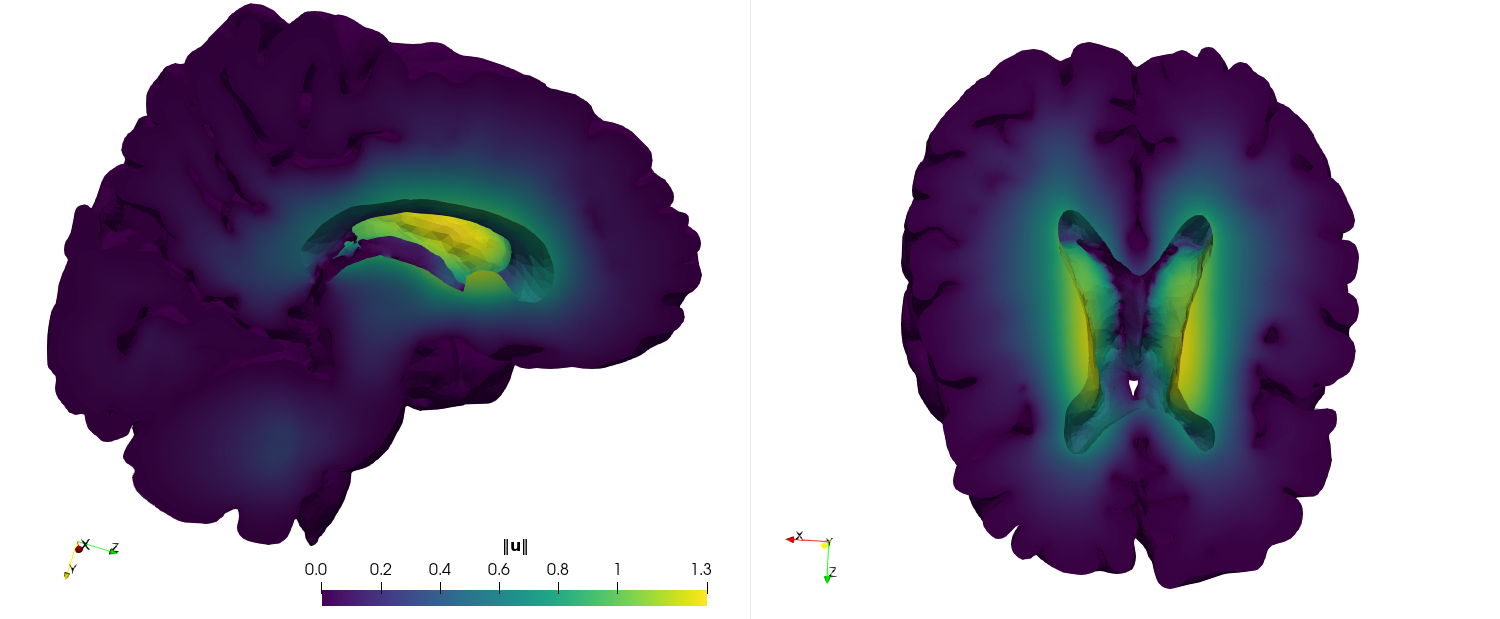
\includegraphics[width=\textwidth]{figures/brain_pressure.png}
\end{minipage}\hfill
\begin{minipage}[t]{4in}
\vspace{5mm}
\textbf{$\triangleleft$ Figure:}
A pressure of 3 mmHg applied to the ventricular surface and the force balance equations are solved using FEniCSx. Colormap show resulting magnitude of the displacement field.
\end{minipage}



\end{minipage}};

\node[anchor=east, rounded corners=3mm, fill=simula]
(drug title)
at ($ (drug.north east)!3cm!(drug.north west) $)
{\ffmfamily Inverse estimation of pressure};



%%%% References %%%%

\node[draw=none, anchor=north west]
(references)
at ($(drug.south west)+(0,-0.7cm)$)
{\begin{minipage}{10.5in}


\begin{minipage}[t]{\textwidth}

{\bfseries\ffmfamily\Large\underline{References}}
\vfill
\vspace{0.2cm}
\footnotesize
[1] Holland, Dominic, et al. "Nonlinear registration of longitudinal images and measurement of change in regions of interest." Medical image analysis 15.4 (2011): 489-497. DOI: 10.1016/j.media.2011.02.005

\medskip
[2] Hu, Yixin, et al. "Fast tetrahedral meshing in the wild." ACM Transactions on Graphics (ToG) 39.4 (2020): 117-1. DOI: 10.1145/3386569.3392385

\medskip
[3] Baratta, Igor A., et al. "DOLFINx: the next generation FEniCS problem solving environment." (2023). DOI: 10.5281/zenodo.10447666

\medskip
[4] Petersen, Ronald C., et al. "Mild cognitive impairment: clinical characterization and outcome." Archives of neurology 56.3 (1999): 303-308. DOI: 10.1001/archneur.56.3.303

\medskip
[5] Blinkouskaya et. al. "Brain shape changes associated with cerebral atrophy in healthy aging and Alzheimer’s disease." Frontiers in Mechanical Engineering 7 (2021): 705653. DOI: 10.3389/fmech.2021.705653 
\end{minipage}



\end{minipage}};



%%%% footer %%%%
\begingroup
\pgfmathsetseed{31417}
\fill[simula,
      drop shadow={shadow yshift=1ex, shadow xshift=-1ex}]
decorate[decoration={random steps, segment length=1cm, amplitude=4mm}]
{ ($(current bounding box.south west)+(-1cm,4cm)$) --
  ($(current bounding box.south east)+(1cm,4cm)$) }
-- (current bounding box.south east) --
   (current bounding box.south west) -- cycle;
\node[anchor=west]
at ( $(current bounding box.south west)+(1cm,2cm)$ )
{
\includegraphics[height=2cm]{simula_logo_main_black}};
\node[anchor=east]
at ( $(current bounding box.south east)+(-1cm,2cm)$ )
{
\includegraphics[height=3cm]{KGJcentre_logo_black}};
\endgroup

\end{tikzpicture}

\end{document}
